\documentclass{beamer}
\usepackage[utf8]{inputenc}

\usetheme{Madrid}
\usecolortheme{default}
\usepackage{amsmath,amssymb,amsfonts,amsthm}
\usepackage{txfonts}
\usepackage{tkz-euclide}
\usepackage{listings}
\usepackage{adjustbox}
\usepackage{array}
\usepackage{tabularx}
\usepackage{gvv}
\usepackage{lmodern}
\usepackage{circuitikz}
\usepackage{tikz}
\usepackage{graphicx}

\setbeamertemplate{page number in head/foot}[totalframenumber]

\usepackage{tcolorbox}
\tcbuselibrary{minted,breakable,xparse,skins}



\definecolor{bg}{gray}{0.95}
\DeclareTCBListing{mintedbox}{O{}m!O{}}{%
  breakable=true,
  listing engine=minted,
  listing only,
  minted language=#2,
  minted style=default,
  minted options={%
    linenos,
    gobble=0,
    breaklines=true,
    breakafter=,,
    fontsize=\small,
    numbersep=8pt,
    #1},
  boxsep=0pt,
  left skip=0pt,
  right skip=0pt,
  left=25pt,
  right=0pt,
  top=3pt,
  bottom=3pt,
  arc=5pt,
  leftrule=0pt,
  rightrule=0pt,
  bottomrule=2pt,

  colback=bg,
  colframe=orange!70,
  enhanced,
  overlay={%
    \begin{tcbclipinterior}
    \fill[orange!20!white] (frame.south west) rectangle ([xshift=20pt]frame.north west);
    \end{tcbclipinterior}},
  #3,
}
\lstset{
    language=C,
    basicstyle=\ttfamily\small,
    keywordstyle=\color{blue},
    stringstyle=\color{orange},
    commentstyle=\color{green!60!black},
    numbers=left,
    numberstyle=\tiny\color{gray},
    breaklines=true,
    showstringspaces=false,
}
%------------------------------------------------------------
%This block of code defines the information to appear in the
%Title page
\title %optional
{4.8.27}
\date{\today}
%\subtitle{A short story}

\author % (optional)
{Shivam Sawarkar \\ AI25BTECH11031}



\begin{document}


\frame{\titlepage}
\begin{frame}{Question}
    Find the equation of the plane passing through $(-1, 3, 2)$ and perpendicular to the planes $x + 2y + 3z = 5$ and $3x + 3y + z = 0$.
\end{frame}

\begin{frame}{Solution}
    Normals of the given planes are
\begin{align}
\vec{n_1} = \myvec{1 \\ 2 \\ 3},
\quad
\vec{n_2} = \myvec{3 \\ 3 \\ 1}.
\end{align}

Let the required plane have normal vector $\vec{n}$

Since it is perpendicular to both given planes:
\begin{align}
\vec{n_1}^\top \vec{n} = 0,
\quad
\vec{n_2}^\top \vec{n} = 0.
\end{align}
That is,
\begin{align}
\myvec{\vec{n_1} & \vec{n_2}}^\top\vec{n}=\myvec{0 \\ 0} \\ 
\myvec{
1 & 2 & 3 \\
3 & 3 & 1
}
\vec{n}
=
\myvec{
0 \\ 0
}.
\end{align}
\end{frame}

\begin{frame}{Solution}
    Let
\begin{align}
\vec{n} = \myvec{a \\ b \\ c} \\ 
a + 2b + 3c = 0, \\
3a + 3b + c = 0.
\end{align}

From these, we get
\begin{align}
\vec{n} = t \myvec{7 \\ -8 \\ 3}, \quad t \in \mathbb{R}, \quad t \neq 0
\end{align}

Equation of plain is 
\begin{align}
    \vec{n}^\top\vec{x}=1
\end{align}
\end{frame}

\begin{frame}{Solution}
    since point $\vec{p}=\myvec{-1 \\ 3 \\ 2}$ lies on the plain
\begin{align}
    \vec{n}^\top\vec{p}=1
\end{align}

Substituting,
\begin{align}
\myvec{7 & -8 & 3}
\myvec{x \\ y \\ z}
=
\myvec{7 & -8 & 3}\myvec{-1 \\ 3 \\ 2}.
\end{align}
\end{frame}

\begin{frame}{Solution}
    Substituting,
\begin{align}
\myvec{7 & -8 & 3}
\myvec{x \\ y \\ z}
=
\myvec{7 & -8 & 3}\myvec{-1 \\ 3 \\ 2}.
\end{align}

\begin{align}
\myvec{7 & -8 & 3}
\myvec{x \\ y \\ z}
= -25
\end{align}

\begin{align}
\frac{-1}{25}\myvec{7 & -8 & 3}
\myvec{x \\ y \\ z}
=1 
\end{align}

\begin{align}
\vec{n}=\frac{-1}{25}\myvec{7 \\ -8 \\ 3}
\end{align}
\end{frame}

\begin{frame}{Plot}
    \begin{figure}
        \centering
        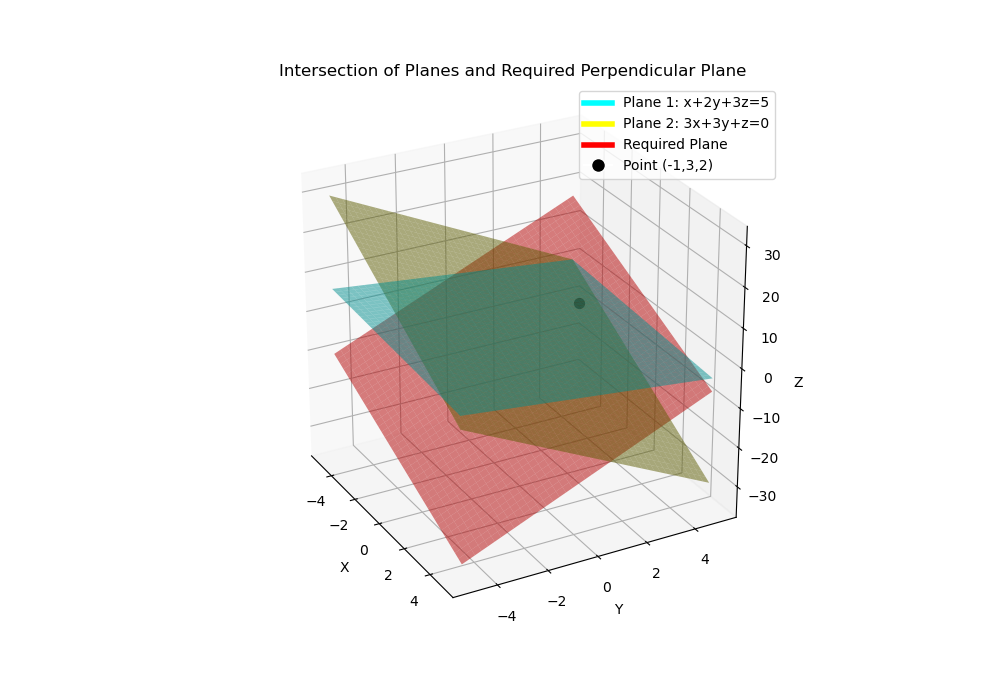
\includegraphics[width=1\linewidth]{figs/plot8.png}
        \caption{}
        \label{fig:placeholder}
    \end{figure}
\end{frame}

\begin{frame}[fragile]{C Code}
    \begin{verbatim}
#ifndef PLANE_H
#define PLANE_H

#include <stdio.h>

// Function to compute cross product of two vectors
void cross_product(double a1, double b1, double c1,
                   double a2, double b2, double c2,
                   double *rx, double *ry, double *rz) {
    *rx = b1*c2 - c1*b2;
    *ry = c1*a2 - a1*c2;
    *rz = a1*b2 - b1*a2;
}
    \end{verbatim}
\end{frame}

\begin{frame}[fragile]{C Code}
    \begin{verbatim}
// Function to compute dot product of two vectors
double dot_product(double a1, double b1, double c1,
                 double a2, double b2, double c2) {
  return a1*a2 + b1*b2 + c1*c2;
}

// Function to print plane equation given normal and point
void plane_equation(double nx, double ny, double nz,
                  double x0, double y0, double z0) {
  double rhs = dot_product(nx, ny, nz, x0, y0, z0);
  printf("\nEquation of required plane: %.2lf*x + %.2lf*y + %.2lf*z = %.2lf\n",
         nx, ny, nz, rhs);
}

#endif
    \end{verbatim}
\end{frame}

\begin{frame}[fragile]{C Code}
    \begin{verbatim}
#include "solution.h"

int main() {
    double x0, y0, z0;
    printf("Enter point (x0 y0 z0): ");
    scanf("%lf %lf %lf", &x0, &y0, &z0);
    double a1, b1, c1, d1;
    printf("Enter coefficients of plane1 (a1 b1 c1 d1): ");
    scanf("%lf %lf %lf %lf", &a1, &b1, &c1, &d1);
    double a2, b2, c2, d2;
    printf("Enter coefficients of plane2 (a2 b2 c2 d2): ");
    scanf("%lf %lf %lf %lf", &a2, &b2, &c2, &d2);

    // Normal vectors of plane1 and plane2
    double n1x = a1, n1y = b1, n1z = c1;
    double n2x = a2, n2y = b2, n2z = c2;
    \end{verbatim}
\end{frame}

\begin{frame}[fragile]{C Code}
    \begin{verbatim}
    // Compute required normal (cross product)
    double nx, ny, nz;
    cross_product(n1x, n1y, n1z, n2x, n2y, n2z, &nx, &ny, &nz);

    // Print required plane
    plane_equation(nx, ny, nz, x0, y0, z0);

    return 0;
}
    \end{verbatim}
\end{frame}

\begin{frame}[fragile]{Python Code}
    \begin{verbatim}
import numpy as np

def cross_product(v1, v2):
    """Return cross product of two vectors"""
    return np.cross(v1, v2)

def dot_product(v1, v2):
    """Return dot product of two vectors"""
    return np.dot(v1, v2)

def plane_equation(normal, point):
    """Given normal vector and point, return plane equation coefficients"""
    d = dot_product(normal, point)
    return (*normal, d)
    \end{verbatim}
\end{frame}

\begin{frame}[fragile]{Python Code}
    \begin{verbatim}
def main():
    # Input point
    x0, y0, z0 = map(float, input("Enter point (x0 y0 z0): ").split())

    # Input first plane coefficients
    a1, b1, c1, d1 = map(float, input("Enter coefficients of plane1 (a1 b1 c1 d1): ").split())

    # Input second plane coefficients
    a2, b2, c2, d2 = map(float, input("Enter coefficients of plane2 (a2 b2 c2 d2): ").split())

    # Normals of plane1 and plane2
    n1 = np.array([a1, b1, c1])
    n2 = np.array([a2, b2, c2])

    # Required normal vector is cross product
    n_required = cross_product(n1, n2)
    \end{verbatim}
\end{frame}

\begin{frame}[fragile]{Python Code}
    \begin{verbatim}
    # Given point
    p = np.array([x0, y0, z0])

    # Plane equation: n·x = d
    a, b, c, d = plane_equation(n_required, p)

    print(f"\nRequired plane equation:")
    print(f"{a:.2f}x + {b:.2f}y + {c:.2f}z = {d:.2f}")

if __name__ == "__main__":
    main()
    \end{verbatim}
\end{frame}

\begin{frame}[fragile]{Python + C Code}
    \begin{verbatim}
import ctypes
import numpy as np

plane_lib = ctypes.CDLL("./solution.so")

plane_lib.cross_product.argtypes = [
    ctypes.c_double, ctypes.c_double, ctypes.c_double,
    ctypes.c_double, ctypes.c_double, ctypes.c_double,
    ctypes.POINTER(ctypes.c_double), ctypes.POINTER(ctypes.c_double), ctypes.POINTER(ctypes.c_double)
]
plane_lib.cross_product.restype = None

plane_lib.dot_product.argtypes = [
    ctypes.c_double, ctypes.c_double, ctypes.c_double,
    ctypes.c_double, ctypes.c_double, ctypes.c_double
]
    \end{verbatim}
\end{frame}

\begin{frame}[fragile]{Python + C Code}
    \begin{verbatim}
plane_lib.dot_product.restype = ctypes.c_double

plane_lib.plane_equation.argtypes = [
    ctypes.c_double, ctypes.c_double, ctypes.c_double,
    ctypes.c_double, ctypes.c_double, ctypes.c_double
]
plane_lib.plane_equation.restype = None


def main():
    x0, y0, z0 = map(float, input("Enter point (x0 y0 z0): ").split())
    a1, b1, c1, d1 = map(float, input("Enter coefficients of plane1 (a1 b1 c1 d1): ").split())
    a2, b2, c2, d2 = map(float, input("Enter coefficients of plane2 (a2 b2 c2 d2): ").split())
    \end{verbatim}
\end{frame}

\begin{frame}[fragile]{Python + C Code}
    \begin{verbatim}
    n1x, n1y, n1z = a1, b1, c1
    n2x, n2y, n2z = a2, b2, c2

    nx = ctypes.c_double()
    ny = ctypes.c_double()
    nz = ctypes.c_double()
    plane_lib.cross_product(n1x, n1y, n1z, n2x, n2y, n2z,
    ctypes.byref(nx), ctypes.byref(ny), ctypes.byref(nz))

    rhs = plane_lib.dot_product(nx.value, ny.value, 
    nz.value, x0, y0, z0)

    print(f"\nRequired plane equation:")
    print(f"{nx.value:.2f}x + {ny.value:.2f}y + 
    {nz.value:.2f}z = {rhs:.2f}")
    \end{verbatim}
\end{frame}






\end{document}